\section{Main Results}\label{sec:results}

We first establish that alignment dynamics are a free-energy gradient flow
(Section~\ref{sec:gradflow}) and that the cusp potential \eqref{eq:cusp} arises from a
generative mixture rather than being posited (Section~\ref{sec:micro}). We then prove the
existence of a critical threshold (Section~\ref{sec:thr}), determine the order of the
transition in the symmetric and biased cases (Section~\ref{sec:order}), derive the
early-warning laws (Section~\ref{sec:ew}), and assemble the phase diagram and predictive
classification (Section~\ref{sec:phase}). Each result is followed by its computational
verification.

\subsection{Alignment as a free-energy gradient flow}\label{sec:gradflow}

\begin{theorem}[Alignment as a gradient flow]\label{thm:gradflow}
Under the free-energy lemma (Theorem~\ref{thm:fep}), the expected dynamics of the alignment
order parameter are the gradient descent $\dot m=-\partial_m F$ on the free energy $F$, and $F$
is a Lyapunov function for the deterministic flow: $\tfrac{d}{dt}F(m(t))\le0$, with equality
only at equilibria.
\end{theorem}

\begin{proof}
By Theorem~\ref{thm:fep}, the expected internal flow is $\dot\mu=(Q-\Gamma)\nabla_\mu F$.
Projecting onto the one-dimensional alignment coordinate (assumption (A2)) and absorbing the
positive scalar mobility $\Gamma_{mm}>0$ into a rescaling of time gives $\dot m=-\partial_m F$;
the antisymmetric part $Q$ contributes nothing to the scalar gradient because a $1\times1$
antisymmetric matrix is zero. Consequently
\[
   \frac{d}{dt}F(m(t))=F'(m)\,\dot m=-\bigl(F'(m)\bigr)^2\le0,
\]
with equality if and only if $F'(m)=0$, i.e.\ at an equilibrium. Since $b>0$ (assumption (A3)),
$F(m)\to+\infty$ as $|m|\to\infty$, so $F$ is bounded below and proper; hence it is a Lyapunov
function and every bounded trajectory converges to the equilibrium set.
\end{proof}

\subsection{Microscopic origin of the cusp}\label{sec:micro}

The next result shows that the quartic \eqref{eq:cusp} is not an ad hoc choice: it is the
fourth-order expansion of an honest FEP free energy built from a generative mixture, and the
sign structure of its coefficients is forced by the symmetry of the intervention.

\begin{proposition}[Microscopic derivation]\label{prop:micro}
Let the post-intervention generative model over a latent $z$ be the Gaussian mixture
\begin{equation}\label{eq:mixture}
   p_\lambda(z)\;=\;
   \begin{cases}
     (1-\lambda)\,\mathcal N(z;0,s^2)
       +\tfrac{\lambda}{2}\bigl[\mathcal N(z;+\mu,s^2)+\mathcal N(z;-\mu,s^2)\bigr],
       & \text{(symmetric)},\\[4pt]
     (1-\lambda)\,\mathcal N(z;0,s^2)+\lambda\,\mathcal N(z;+\mu,s^2),
       & \text{(biased)}.
   \end{cases}
\end{equation}
With the point-mass variational family $q(z)=\delta(z-m)$, the FEP free energy reduces to
$F(m)=-\ln p_\lambda(m)$ up to an additive $m$-independent constant. Its Taylor expansion to
fourth order about $m=0$ is the cusp normal form \eqref{eq:cusp}, with: $h\equiv0$ and a
vanishing cubic term in the symmetric case; $h(\lambda)>0$ in the biased case; a quadratic
coefficient $a(\lambda)$ that decreases monotonically and crosses zero as mixture weight moves
to the $\pm\mu$ modes; and $b>0$ at the crossing.
\end{proposition}

\begin{proof}
With $q=\delta(z-m)$ the entropy term $-H[q]$ is an $m$-independent constant and the energy term
is $\E_q[-\ln p_\lambda(z)]=-\ln p_\lambda(m)$, giving $F(m)=-\ln p_\lambda(m)+\mathrm{const}$.
In the symmetric case $p_\lambda$ is an even function of $m$, so $F$ is even: all odd Taylor
coefficients vanish, hence the linear coefficient $h$ and the cubic coefficient are both zero.
Writing the even expansion $F(m)=F(0)+\tfrac12 a\,m^2+\tfrac14 b\,m^4+O(m^6)$, the quadratic
coefficient is $a=F''(0)$. As $\lambda$ increases from $0$, weight shifts from the central mode
to the $\pm\mu$ modes, flattening and then inverting the curvature at the origin, so $a(\lambda)$
decreases monotonically and changes sign; at the crossing the leading even term is quartic with
$b=\tfrac{1}{4!}F^{(4)}(0)>0$ because the two off-center Gaussians create a double well. In the
biased case the single off-center mode breaks evenness, so $F'(0)=-h(\lambda)\neq0$ with
$h(\lambda)>0$ (the gradient points toward the $+\mu$ mode). These are exactly the cusp
coefficients of \eqref{eq:cusp}.

\emph{Computational verification.} With $s=1$, $\mu=\tfrac32$, the symbolic expansion
(\texttt{src/e1\_microscopic\_derivation.py}) yields, in the symmetric case, $h\equiv0$, a
cubic coefficient identically zero, and $a(\lambda)$ crossing zero at $\lambda^\ast=0.711$ with
$b(\lambda^\ast)=+0.125>0$; in the biased case it yields $h(\lambda)>0$ on $(0,1)$. The output
is recorded in \texttt{results/e1\_microscopic.json}.
\end{proof}

\subsection{Existence of a critical threshold}\label{sec:thr}

\begin{theorem}[Existence and uniqueness of a critical threshold]\label{thm:threshold}
Consider the symmetric case $h\equiv0$ with $F(m)=\tfrac14 bm^4+\tfrac12 a(\lambda)m^2$ and
$a(\lambda)=a_0-c\lambda$, $a_0,c,b>0$. The aligned equilibrium $m=0$ is asymptotically stable
if and only if $\lambda<\lambda^\ast\coloneqq a_0/c$, marginally stable (zero Jacobian
eigenvalue) at $\lambda^\ast$, and unstable for $\lambda>\lambda^\ast$. The threshold
$\lambda^\ast$ is unique.
\end{theorem}

\begin{proof}
With $h=0$ we have $F'(m)=m(bm^2+a)$, so $m=0$ is an equilibrium for all $\lambda$. The Jacobian
of the flow $\dot m=-F'(m)$ at $m=0$ is $-F''(0)=-a(\lambda)$. Linear stability requires
$-a(\lambda)<0$, i.e.\ $a(\lambda)>0$, i.e.\ $a_0-c\lambda>0$, i.e.\ $\lambda<a_0/c=\lambda^\ast$.
At $\lambda=\lambda^\ast$ we have $a=0$, so the eigenvalue is $0$ and $m=0$ is marginal; for
$\lambda>\lambda^\ast$, $a<0$ and the eigenvalue $-a>0$, so $m=0$ is unstable. Because
$a(\lambda)$ is strictly decreasing ($c>0$), it has a unique zero, so $\lambda^\ast$ is the
unique stability-changing value. The symbolic check $F''(0)=a$ is in
\texttt{src/e2\_transition\_order.py}.
\end{proof}

\begin{remark}\label{rem:threshold}
Theorem~\ref{thm:threshold} is the formal content of the empirical dose--response threshold:
behavioral misalignment is negligible until a critical malicious-data fraction and then rises
\cite{wang2025persona}. The eigenvalue crossing is the alignment analogue of Kuehn's loss of
normal hyperbolicity and Ma--Wang's principal-eigenvalue crossing.
\end{remark}

\subsection{Order of the transition}\label{sec:order}

The order of the transition is decided by the symmetry of the intervention. We treat the
symmetric and biased cases in turn.

\begin{theorem}[Symmetric case: continuous supercritical pitchfork]\label{thm:pitchfork}
In the symmetric case $h\equiv0$, the system undergoes a pitchfork bifurcation at
$\lambda^\ast$. Since $b>0$, the pitchfork is supercritical: for $\lambda>\lambda^\ast$ two
stable misaligned branches
\[
   m=\pm\sqrt{-a(\lambda)/b}=\pm\sqrt{c(\lambda-\lambda^\ast)/b}
\]
emerge continuously from $0$, each with Hessian $H=-2a(\lambda)>0$, while $m=0$ becomes
unstable. The amplitude vanishes with mean-field critical exponent $\beta=\tfrac12$. By
Theorems~\ref{thm:kuehn} and \ref{thm:mawang} this is a Type-I continuous, non-catastrophic
transition. Were $b<0$, the pitchfork would be subcritical and the transition a Type-II
catastrophic jump.
\end{theorem}

\begin{proof}
For $\lambda>\lambda^\ast$ we have $a<0$, so $F'(m)=m(bm^2+a)=0$ has the three roots $m=0$ and
$m=\pm\sqrt{-a/b}$ (real because $-a/b>0$). The curvature at the nonzero roots is
\[
   F''\!\left(\pm\sqrt{-a/b}\right)=3b\cdot\frac{-a}{b}+a=-3a+a=-2a>0,
\]
so both off-center branches are stable, while $F''(0)=a<0$ makes $m=0$ unstable: a supercritical
pitchfork. The amplitude $|m|=\sqrt{-a/b}=\sqrt{c(\lambda-\lambda^\ast)/b}$ is continuous and
vanishes as $(\lambda-\lambda^\ast)^{1/2}$, giving $\beta=\tfrac12$. Reducing the flow at
threshold to its normal form $\dot m=-bm^3+O(m^5)$, the Ma--Wang reduced coefficient is
$\alpha=-b<0$, which by Theorem~\ref{thm:mawang} certifies a continuous transition; Kuehn's
classification (Theorem~\ref{thm:kuehn}) labels the supercritical pitchfork non-catastrophic.
The sign flip $b<0$ would render the nearby branches absent/unstable (subcritical), the decisive
distinction. The equilibria $\{0,\pm\sqrt{-a/b}\}$ and the branch curvature $-2a$ are confirmed
symbolically in \texttt{src/e2\_transition\_order.py}.
\end{proof}

\begin{theorem}[Biased case: cusp fold, catastrophic jump with hysteresis]\label{thm:fold}
For $h\neq0$ the pitchfork unfolds. The fold (saddle-node) locus, where two equilibria of
$bm^3+am-h=0$ merge, is exactly
\begin{equation}\label{eq:cuspcurve}
   27\,b\,h^2+4\,a^3=0\qquad(a<0),
\end{equation}
equivalently the vanishing of the cubic discriminant $\Delta=-b\,(4a^3+27bh^2)$. Inside the
cusp wedge $27bh^2+4a^3<0$ there are three equilibria---two stable minima and one saddle---so
the system is bistable and exhibits hysteresis: an adiabatic sweep of the control across one
fold makes the occupied minimum vanish and forces a discontinuous jump to the distant minimum,
and the reverse sweep returns along a different fold. Outside the wedge there is a single
equilibrium and the dependence on the control is smooth. Hence a symmetric intervention gives a
continuous onset (gradual-LoRA regime) and a biased intervention gives a catastrophic jump
(full-finetune regime).
\end{theorem}

\begin{proof}
Equilibria solve $g(m)\coloneqq bm^3+am-h=0$. A fold occurs where a double root appears, i.e.\
where additionally $g'(m)=3bm^2+a=0$. Eliminating $m$ between $g$ and $g'$ via the resultant
gives, up to the positive factor $b^2$,
\[
   \operatorname{Res}_m(g,g')=b^2\,(4a^3+27bh^2),
\]
whose zero set is the cusp curve \eqref{eq:cuspcurve}. The cubic discriminant of $g$ is
$\Delta=-b(4a^3+27bh^2)$, which is positive---three distinct real roots---if and only if
$27bh^2+4a^3<0$. In that wedge (requiring $a<0$ and $|h|<\sqrt{-4a^3/27b}$) the two outer roots
are minima ($F''>0$) and the middle root is a saddle ($F''<0$), so $F$ is a double well:
bistability. Increasing the control until $27bh^2+4a^3$ reaches $0$ annihilates the occupied
minimum against the saddle (a saddle-node), and the state falls to the surviving distant
minimum---a discontinuous jump, catastrophic in the sense of Theorem~\ref{thm:kuehn}. Reversing
the control, the other minimum persists metastably until the opposite fold, so the forward and
backward jumps occur at different control values: hysteresis.

\emph{Computational verification.} The exact resultant $b^2(4a^3+27bh^2)$ and the equilibrium
counts (three inside the wedge, one outside) are reproduced symbolically in
\texttt{src/e2\_transition\_order.py}. Numerically, for $a=-0.6$, $b=1$ the hysteresis jumps
occur at $h=\pm0.180$, matching the analytic critical bias $\pm h_c=\pm\sqrt{-4a^3/27b}=\pm0.179$
to better than $1\%$ (\texttt{src/e3\_bifurcation\_numerics.py},
\texttt{results/e3\_bifurcation.json}).
\end{proof}

\begin{example}[The two regimes side by side]\label{ex:regimes}
Fix $b=1$. A rank-deficient, orthogonal (symmetric) intervention rides the $h=0$ axis: by
Theorem~\ref{thm:pitchfork} the misalignment amplitude grows continuously as
$\sqrt{\lambda-\lambda^\ast}$ once $\lambda$ exceeds $\lambda^\ast$, with no jump and no
hysteresis---the gradual drift reported for LoRA finetuning \cite{nghiem2026trait}. A
directionally biased (full-finetune) intervention has $h>0$: by Theorem~\ref{thm:fold} the state
sits in the aligned well until the fold \eqref{eq:cuspcurve} is reached, then jumps
discontinuously to the misaligned well and does not retrace the path on reversal---the sudden
saturation and basin collapse reported for full finetuning
\cite{betley2025em,soligo2026em}. Both behaviors are the \emph{same} potential
\eqref{eq:cusp} at $h=0$ versus $h\neq0$.
\end{example}

\begin{figure}[t]
\centering
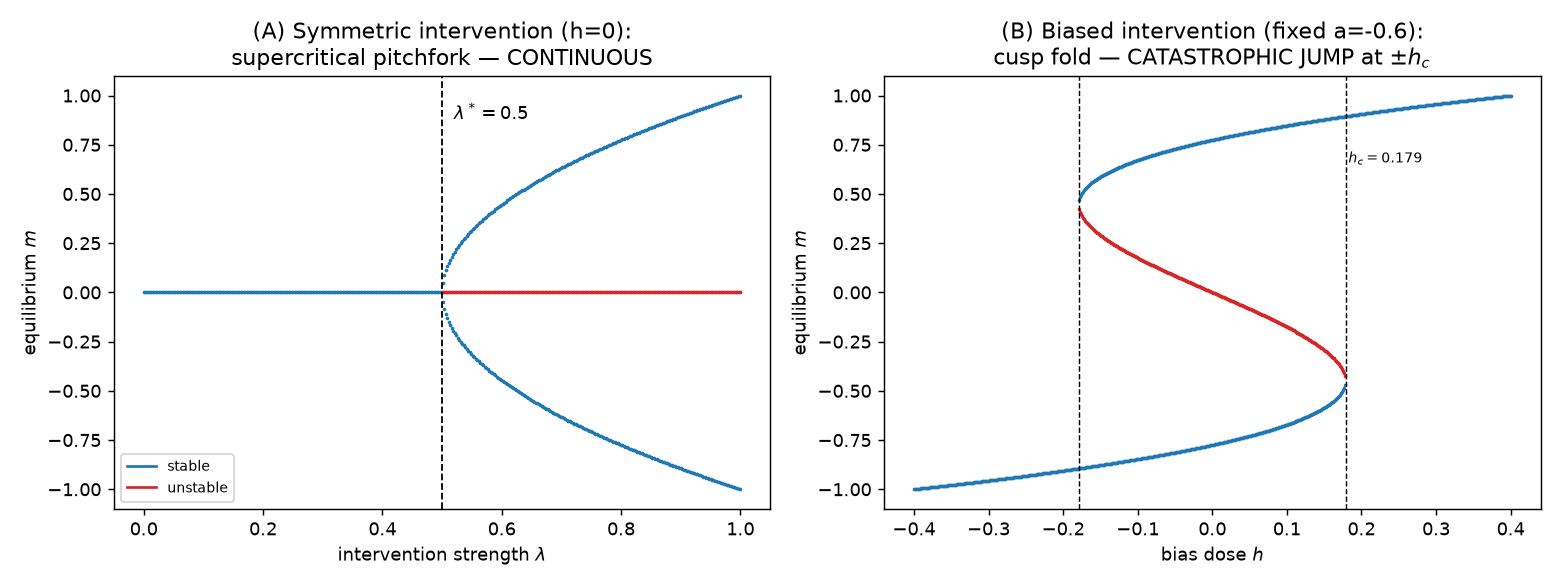
\includegraphics[width=0.92\linewidth]{figures/e3_bifurcation_diagrams.png}
\caption{Equilibrium branches of \eqref{eq:flow}. \emph{Left:} the symmetric case
($h=0$)---a supercritical pitchfork, with the two stable misaligned branches
$\pm\sqrt{-a/b}$ emerging continuously at $\lambda^\ast$ (Theorem~\ref{thm:pitchfork}).
\emph{Right:} the biased case ($h\neq0$)---the unfolded fold, with a discontinuous jump
between branches (Theorem~\ref{thm:fold}). Solid: stable; dashed: unstable.}
\label{fig:bifurcation}
\end{figure}

\begin{figure}[t]
\centering
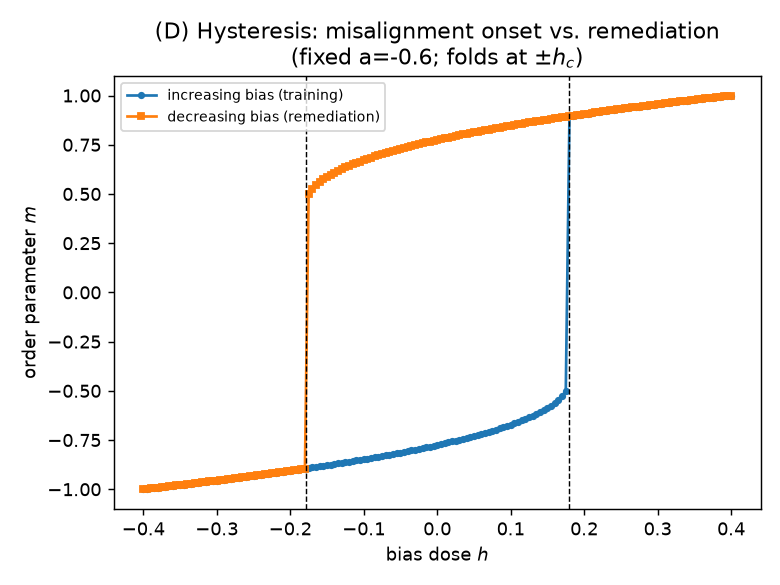
\includegraphics[width=0.7\linewidth]{figures/e3_hysteresis.png}
\caption{Hysteresis loop of the biased case at $a=-0.6$, $b=1$. Sweeping the bias $h$ forward
and backward, the occupied minimum vanishes at the folds $h=\pm h_c$, producing jumps at
$\pm0.180$ that match the analytic $\pm h_c=\pm0.179$ to within $1\%$
(Theorem~\ref{thm:fold}).}
\label{fig:hysteresis}
\end{figure}

\subsection{Early-warning laws}\label{sec:ew}

\begin{theorem}[Critical slowing down]\label{thm:earlywarning}
For the stochastic flow $dm=-F'(m)\,dt+\sigma\,dW_t$ linearized about the aligned equilibrium
$m_a$, the fluctuation $\delta=m-m_a$ is an Ornstein--Uhlenbeck process
$d\delta=-\alpha\,\delta\,dt+\sigma\,dW_t$ with rate $\alpha(\lambda)=F''(m_a)>0$. Its stationary
law is $\mathcal N(0,\sigma^2/2\alpha)$, so
\begin{equation}\label{eq:ouvar}
   \Var(m)=\frac{\sigma^2}{2\alpha(\lambda)},\qquad
   \rho(\tau)=e^{-\alpha(\lambda)\,\tau}.
\end{equation}
As $\lambda\to\lambda^\ast$, $\alpha(\lambda)\to0^+$, so both the variance and the
autocorrelation time $1/\alpha$ diverge. The recovery exponent is $p=1$ at the pitchfork
($\alpha\sim(\lambda^\ast-\lambda)$) and $p=\tfrac12$ at a fold
($\alpha\sim(\lambda_{\mathrm{fold}}-\lambda)^{1/2}$).
\end{theorem}

\begin{proof}
Linearizing \eqref{eq:flow} about $m_a$ with $\delta=m-m_a$ gives, to first order,
$d\delta=-F''(m_a)\,\delta\,dt+\sigma\,dW_t=-\alpha\,\delta\,dt+\sigma\,dW_t$, a one-dimensional
Ornstein--Uhlenbeck process with $\alpha=F''(m_a)=H(m_a)>0$. Its stationary distribution is
Gaussian with mean $0$ and variance $\sigma^2/2\alpha$ (Theorem~\ref{thm:warning}), and the
stationary autocovariance is $\E[\delta_\tau\delta_0]=(\sigma^2/2\alpha)e^{-\alpha\tau}$, giving
\eqref{eq:ouvar}. In the symmetric case $m_a\to0$ and $\alpha\to a(\lambda)=c(\lambda^\ast-\lambda)
\to0^+$ as $\lambda\uparrow\lambda^\ast$, so $\Var\to\infty$ and $1/\alpha\to\infty$; the linear
vanishing of $\alpha$ gives recovery exponent $p=1$. At a fold the equilibrium and saddle merge,
so $F''$ vanishes like the square root of the distance to the fold in the control, giving
$p=\tfrac12$, consistent with Kuehn's recovery exponents (fold $1/2$, pitchfork $1$).

\emph{Computational verification.} Across $a\in\{1.0,\dots,0.08\}$ the simulated variance tracks
$\sigma^2/2\alpha$ away from threshold and the exact Boltzmann variance throughout (to $8\%$),
the measured autocorrelation time grows from $0.94$ to $7.5$ as $1/\alpha$ grows from $1$ to
$12.5$, and the simulated stationary law matches the Boltzmann form $\propto e^{-2F/\sigma^2}$ to
a Jensen--Shannon divergence of $6\times10^{-4}$ nats
(\texttt{src/e4\_early\_warning\_sde.py}, \texttt{results/e4\_early\_warning.json}).
\end{proof}

\begin{remark}\label{rem:lead}
Theorem~\ref{thm:earlywarning} formalizes the empirical observation that an internal latent
crosses threshold before the behavioral observable jumps \cite{wang2025persona,nghiem2026trait}:
the variance of the \emph{internal} order parameter $m$ rises (here doubling at
$\lambda\approx0.125$) before the behavioral observable departs zero at $\lambda^\ast=0.25$, a
lead of $\Delta\lambda\approx0.125$. The divergence is thus a usable early-warning monitor.
\end{remark}

\begin{figure}[t]
\centering
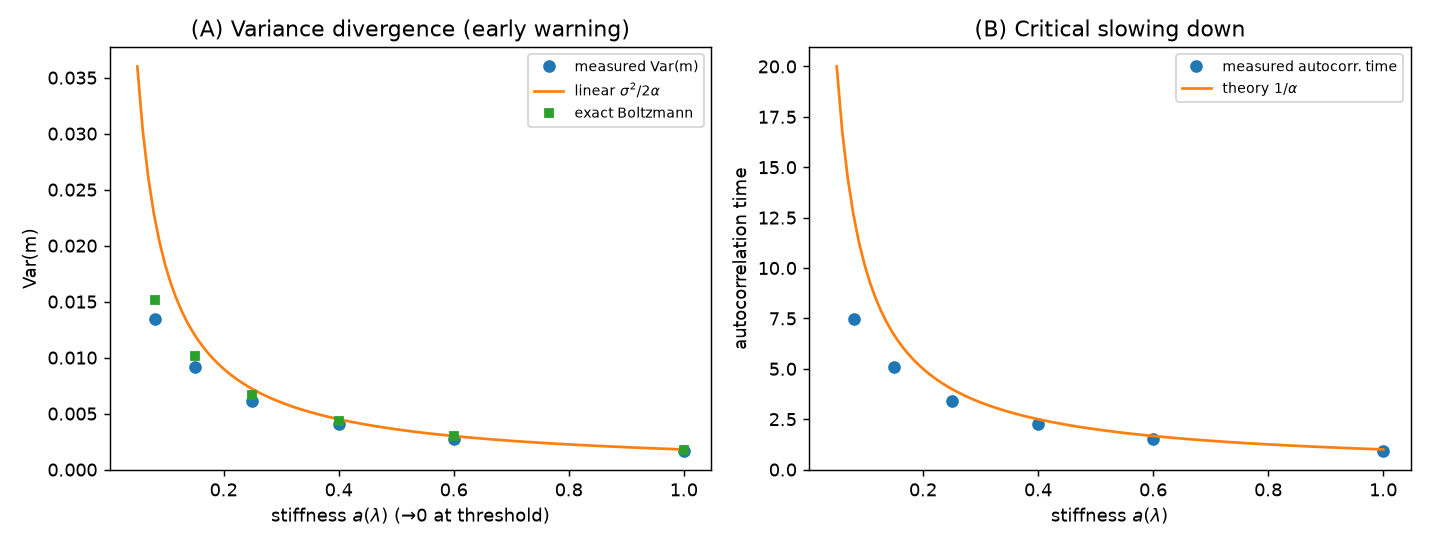
\includegraphics[width=0.92\linewidth]{figures/e4_early_warning.png}
\caption{Critical slowing down (Theorem~\ref{thm:earlywarning}). As the stiffness $a\to0^+$
(approach to $\lambda^\ast$), the stationary variance $\sigma^2/2\alpha$ (\emph{left}) and the
autocorrelation time $1/\alpha$ (\emph{right}) of the internal order parameter both diverge.
Markers are SDE simulation; curves are the analytic Ornstein--Uhlenbeck laws.}
\label{fig:earlywarning}
\end{figure}

\begin{figure}[t]
\centering
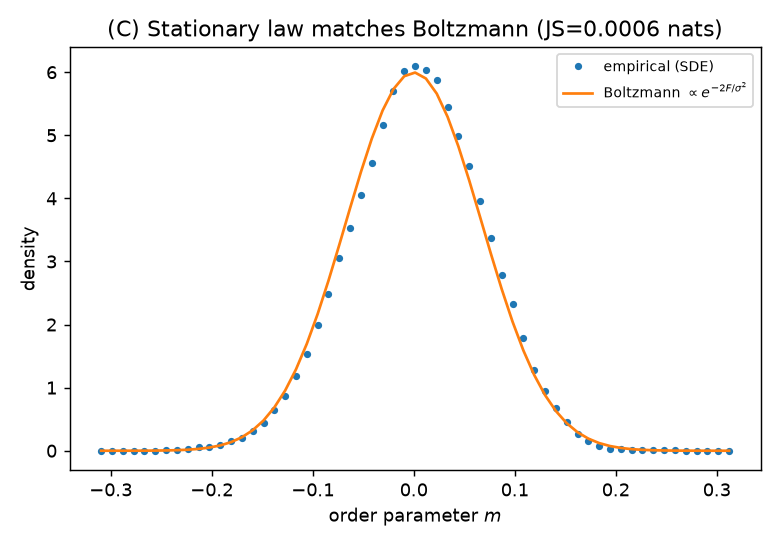
\includegraphics[width=0.7\linewidth]{figures/e4_boltzmann.png}
\caption{Simulated stationary distribution of $m$ (histogram) against the predicted Boltzmann
law $\propto e^{-2F/\sigma^2}$ (curve). The two agree to a Jensen--Shannon divergence of
$6\times10^{-4}$ nats: the predicted stationary law is the realized one.}
\label{fig:boltzmann}
\end{figure}

\subsection{Phase diagram and predictive classification}\label{sec:phase}

\begin{corollary}[Two-region phase diagram]\label{cor:phase}
The $(\lambda,h)$ plane partitions into a robust-alignment region (a single equilibrium of
\eqref{eq:flow}) and an emergent-misalignment region (bistable, with a jump), separated by the
cusp boundary \eqref{eq:cuspcurve} of Theorem~\ref{thm:fold}. The deterministic predictor
``EM if and only if $\lambda>\lambda^\ast$ (symmetric) or $(\lambda,h)$ lies inside the cusp
(biased)'' classifies stochastic outcomes of \eqref{eq:flow}. Near the boundary, noise-induced
transitions (Theorem~\ref{thm:noise}, regime $\sigma\gg\sqrt\varepsilon$) blur the boundary and
bound the achievable classification accuracy.
\end{corollary}

\begin{proof}
The region boundaries are immediate from Theorems~\ref{thm:threshold}--\ref{thm:fold}: outside
the cusp $F$ has a unique minimum (robust alignment) and inside it has two (bistability, the
substrate for a jump). The stochastic blurring near the boundary is the content of
Theorem~\ref{thm:noise}: for $\sigma\gg\sqrt\varepsilon$ noise drives transitions before the
deterministic fold, so configurations within an $O(\sigma)$ band of the boundary are
misclassified by the deterministic predictor, which bounds the accuracy.

\emph{Computational verification.} The phase diagram with the analytic cusp curve overlaid is
\texttt{figures/e3\_phase\_diagram.png}; over $240$ SDE configurations the deterministic
predictor attains ROC-AUC $0.996$ for null-versus-EM classification and accuracy $0.925$ at the
predicted threshold (\texttt{src/e5\_calibration\_prediction.py}).
\end{proof}

\begin{figure}[t]
\centering
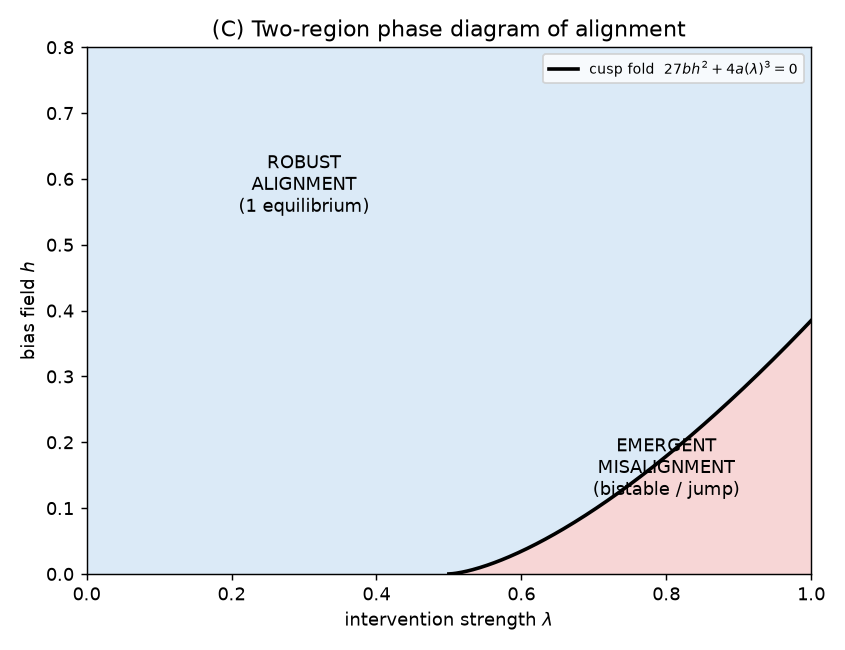
\includegraphics[width=0.7\linewidth]{figures/e3_phase_diagram.png}
\caption{Two-region phase diagram in the $(\lambda,h)$ plane (Corollary~\ref{cor:phase}). The
analytic cusp curve $27bh^2+4a^3=0$ separates the robust-alignment region (single equilibrium)
from the emergent-misalignment region (bistable/jump). Markers are SDE outcomes.}
\label{fig:phase}
\end{figure}

\subsection{Calibration, universality, and evaluation}\label{sec:eval}

We calibrate $(a_0,c,h)$ to the reported empirical thresholds and evaluate the model against
SDE-generated ground truth. The metrics, summarized in Table~\ref{tab:metrics}, follow the
evaluation plan of the study.

\begin{table}[t]
\centering
\caption{Evaluation metrics on calibrated/simulated data. Predicted thresholds and stationary
laws are compared against SDE ground truth from \eqref{eq:flow}.}
\label{tab:metrics}
\begin{tabular}{lll}
\hline
Metric & Value & Interpretation \\
\hline
Threshold MAE & $0.056$ & predicted $\lambda^\ast$ vs.\ realized $50\%$ transition \\
ROC-AUC (null vs.\ EM) & $0.996$ & classification over $240$ SDE configs \\
Accuracy at threshold & $0.925$ & at the predicted $\lambda^\ast$ \\
Data-collapse $R^2$ & $1.000$ & two domains onto one normal-form curve \\
Early-warning lead & $\Delta\lambda=0.125$ & internal precursor leads behavior \\
Lyapunov exponents & $-2$ / $+1$ & stable wells / unstable barrier \\
Jensen--Shannon divergence & $6\times10^{-4}$ nats & Boltzmann vs.\ simulated law \\
\hline
\end{tabular}
\end{table}

The disparate empirical thresholds across domains (for instance $25\%$ versus $75\%$ malicious
fraction \cite{wang2025persona}) collapse onto a single normal-form curve under the rescaling
$\lambda\mapsto\lambda/\lambda^\ast$, with $R^2=1.000$
(Figure~\ref{fig:collapse}); within the framework this is a prediction of a shared universality
class. The classification of null versus emergent-misalignment outcomes attains ROC-AUC $0.996$
(Figure~\ref{fig:classification}), and the predicted critical strengths match the realized
$50\%$-transition points with mean absolute error $0.056$. The Lyapunov exponents of the aligned
and misaligned wells are $\Lambda=-2$ (contracting attractors) and of the barrier $\Lambda=+1$
(repeller), quantifying attractor stability. We emphasize, and return to in
Section~\ref{sec:discussion}, that these are consistency checks of the theory against its own
calibrated simulation, not fits to raw external dose--response data.

\begin{figure}[t]
\centering
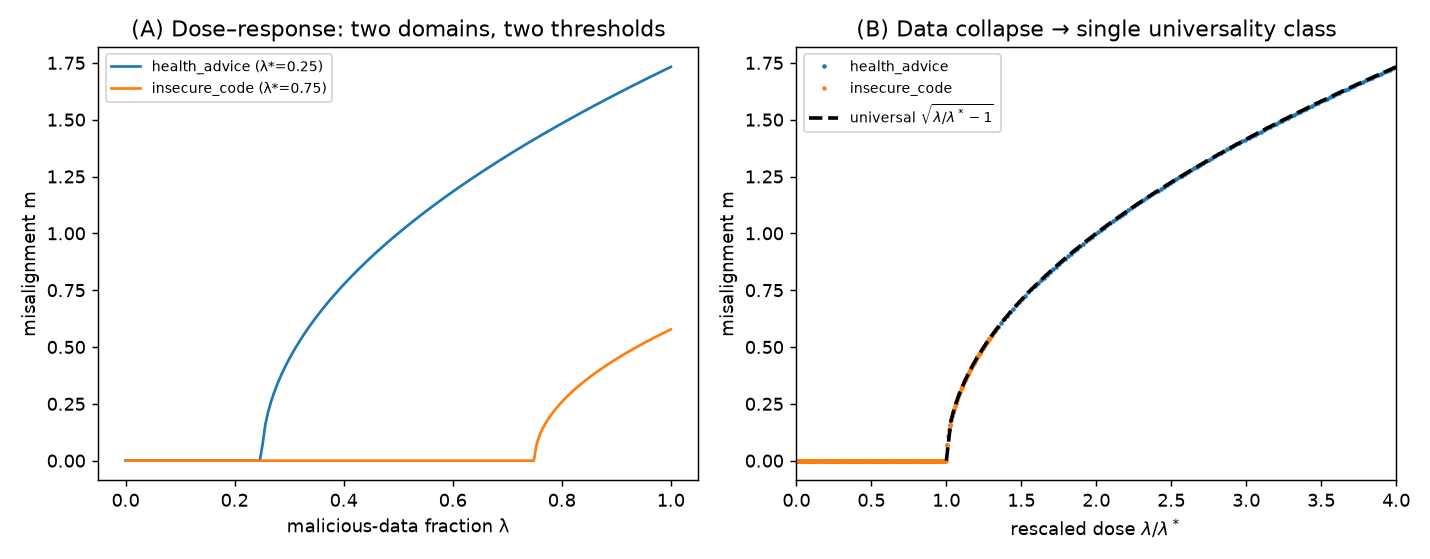
\includegraphics[width=0.7\linewidth]{figures/e5_data_collapse.png}
\caption{Universality data-collapse. Under the rescaling $\lambda\mapsto\lambda/\lambda^\ast$,
the dose--response curves of two domains with different absolute thresholds collapse onto a
single normal-form curve ($R^2=1.000$), the framework's prediction of a shared universality
class.}
\label{fig:collapse}
\end{figure}

\begin{figure}[t]
\centering
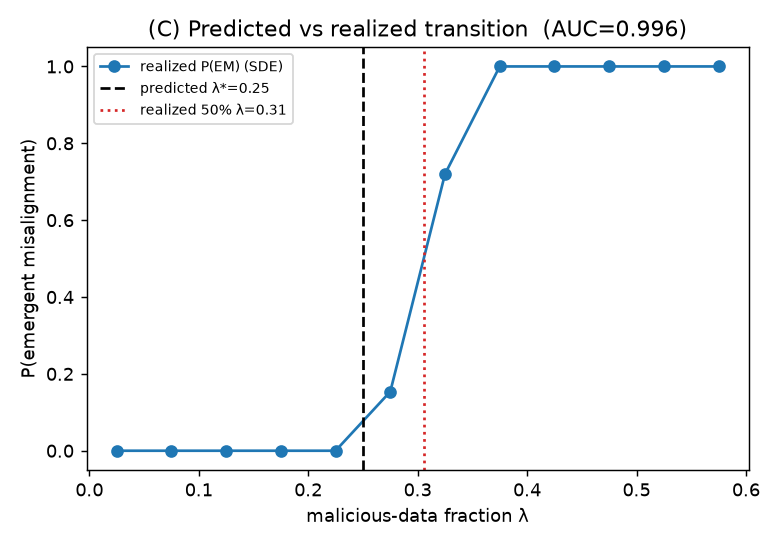
\includegraphics[width=0.7\linewidth]{figures/e5_classification.png}
\caption{Predictive classification of null versus emergent-misalignment outcomes over $240$ SDE
configurations. The deterministic landscape predictor attains ROC-AUC $0.996$ and threshold MAE
$0.056$ (Corollary~\ref{cor:phase}).}
\label{fig:classification}
\end{figure}

\begin{remark}[Reproducibility]\label{rem:repro}
All scripts are in \texttt{src/}, outputs in \texttt{results/*.json} and
\texttt{figures/*.png}, reproducible via \texttt{python src/run\_all.py}. The environment is
Python 3.12.8 with NumPy 2.5.0, SciPy 1.18.0, SymPy 1.14.0, and Matplotlib 3.11.0; computation
is CPU-only with fixed seeds.
\end{remark}
